% Begin the document and set up the style of the document
\documentclass[a4paper,11pt]{article}

% Install the required packages for the document 
\usepackage{enumitem}
\usepackage{amsmath}
\usepackage{amssymb}
\usepackage{verbatim}
\usepackage{mathtools}
\usepackage{tikz}

% Page and style settings
%\parskip=8pt
\parindent=0pt
% Right margin
\textwidth=6.25in
% Left margin
\oddsidemargin=0pt
\evensidemargin=0pt
% Bottom margin
\textheight=10in
% Top margin
\topmargin=-0.75in
\baselineskip=11pt
% end of page and other style settings

\renewcommand{\familydefault}{\sfdefault}
\usepackage{calrsfs}
\DeclareMathAlphabet{\pazocal}{OMS}{zplm}{m}{n}

\newcommand{\indep}{\mathrel{\text{\scalebox{1.07}{$\perp\mkern-10mu\perp$}}}}
\newcommand{\p}{\mathbb{P}}
\newcommand{\e}{\mathbb{E}}
\newcommand{\ds}{\displaystyle}
\newcommand{\code}{\texttt}
\newcommand{\HRule}{\rule{\linewidth}{0.5mm}} % Defines a new command for the horizontal lines, change thickness here

\newenvironment{nscentre}
 {\parskip=0pt\par\nopagebreak\centering}
 {\par\noindent\ignorespacesafterend}


\usepackage{fullpage}

\usepackage{titlesec} % Used to customize the \section command
\titleformat{\section}{\bf}{}{0em}{}[\titlerule] % Text formatting of sections
\titlespacing*{\section}{0pt}{3pt}{3pt} % Spacing around sections

\begin{document}
\setlength{\abovedisplayskip}{8pt}{%
\setlength{\belowdisplayskip}{0pt}{%


\text{School of Mathematics}
\hfill
\text{University of New South Wales}

\begin{nscentre}
	\textbf{MATH2701: Abstract Algebra and Fundamental Analysis}\\
	\textbf{Main Assignment}\\
\end{nscentre}

\text{Name: Keegan Gyoery}
\hfill
\text{zID: z5197058}

\pagenumbering{arabic}
	\begin{enumerate}[leftmargin=*]
		\item Let $\ds{A = \bigl( \begin{smallmatrix}a & b\\ c & d\end{smallmatrix}\bigr) \in {GL}_2(\mathbb{R})}$ and consider the function 
			\begin{align*}
				f_A(x) & = \frac{ax+b}{cx+d}, \hspace{4mm}\text{where $\ds{x}$ is a real number.}
			\end{align*}

			\begin{enumerate}
				\item Assume $\ds{c \neq 0}$. Find the point $\ds{x_0 \in \mathbb{R}}$ at which the function $\ds{f_A}$ is not defined, and find $\ds{y_0 \in \mathbb{R}}$ such that $\ds{y_0 \notin f_A(\mathbb{R} - \{x_0\})}$.
					\bigbreak
					Consider the vertical asymptote $\ds{x = -\frac{d}{c}}$. Let $\ds{x_0 = -\frac{d}{c}}$. Thus, $\ds{f_A(x_0)}$ is clearly undefined. Consider now the horizontal asymptote, found by taking the limit as $\ds{x}$ approaches $\ds{\infty}$, $\ds{y = \frac{a}{c}}$. Let $\ds{y_0 = \frac{a}{c}}$. There does not exist an $\ds{x \in \mathbb{R} - \{x_0\}}$ such that $\ds{f_A(x) = y_0}$. Thus, $\ds{y_0 \notin f_A(\mathbb{R} - \{x_0\})}$.
					\bigbreak

				\item Consider the projective line $\ds{\mathbb{R}P^1 = \mathbb{R}\cup\{\infty\}}$ and assume $\ds{c \neq 0}$. Define $\ds{f_A : \mathbb{R}P^1 \rightarrow \mathbb{R}P^1}$ by
					\begin{align*}
						f_A(x) & = 
						\begin{cases}
							\frac{ax+b}{cx+d}, & \text{if } x \neq x_0, \infty;\\
							\infty 			   & \text{if } x = x_0;\\
							y_0				   & \text{if } x = \infty.\\
						\end{cases}
					\end{align*}
					Show that $\ds{f_A}$ is bijective (i.e., a transformation on $\ds{\mathbb{R}P^1}$).
					\bigbreak
					To prove the above definition for $\ds{f_A}$ is a bijection, we must show that $\ds{f_A}$ is both injective and surjective. For injectivity, we must show that $\ds{f(x_1) = f(x_2) \implies x_1 = x_2}$, so we consider the following three cases.\\
					\textbf{1)} Consider $\ds{f(x_1) = f(x_2) = y_0}$. Thus, $\ds{x_1 = \infty}$ and $\ds{x_2 = \infty}$, so $\ds{x_1 = x_2}$. \\
					\textbf{2)} Consider $\ds{f(x_1) = f(x_2) = \infty}$. Thus, $\ds{x_1 = x_0}$ and $\ds{x_2 = x_0}$, so $\ds{x_1 = x_2}$. \\
					\textbf{3)} Consider $\ds{f(x_1) = f(x_2) \neq y_0, \infty}$. Thus,
					\begin{align*}
						\frac{ax_1 + b}{cx_1 + d} & = \frac{ax_2 + b}{cx_2 + d}\\
						(ax_1 + b)(cx_2 + d) & = (ax_2 + b)(cx_1 + d)\\
						acx_1x_2 + adx_1 + bcx_2 + bd & = acx_1x_2 + adx_2 + bcx_1 + bd\\
						adx_1 + bcx_2 & = adx_2 + bcx_1\\
						(ad - bc)x_1 & = (ad - bc)x_2\\
						\therefore x_1 & = x_2 \hspace{5mm} (ad-bc) \neq 0 \text{ as } A \in GL_2(\mathbb{R}).\\
					\end{align*}
					Clearly, $\ds{f_A}$ is injective, as it is injective for each of the cases, which correspond to the piecewise branches of the definition of $\ds{f_A}$.\\

					\pagebreak

					For surjectivity, we must show that $\ds{\forall y \in \text{im}(f_A), \exists \:x \text{ s.t. } f_A(x) = y}$, so we again consider the same three cases.\\
					\textbf{1)} Consider $\ds{f(x) = y_0}$. Thus, $\ds{x = \infty}$.\\
					\textbf{2)} Consider $\ds{f(x) = \infty}$. Thus, $\ds{x = x_0}$.\\
					\textbf{3)} Consider $\ds{f(x) = \frac{ax+b}{cx+d}}$. Thus,
					\begin{align*}
						f_A(x) & = \frac{ax + b}{cx + d}\\
						(cx + d)f_A(x) & = ax + b\\
						df_A(x) - b & = ax - cxf_A(x)\\
						\therefore x & = \frac{df_A(x) - b}{-cf_A(x) + a}
					\end{align*}
					Note that $\ds{f_A(x) \neq y_0}$ in case \textbf{3)}, as it has been covered in case \textbf{1)}, so there always exists an $\ds{x}$ in the final line of case \textbf{3)}. Clearly, $\ds{f_A}$ is surjective, as it is surjective for each of the cases, which correspond to the piecewise branches of the definition of $\ds{f_A}$. Thus, $\ds{f_A}$ is bijective.
					\bigbreak
				\item If $\ds{c = 0}$, give a definition analogous to (b) for the bijection $\ds{f_A : \mathbb{R}P^1 \rightarrow \mathbb{R}P^1}$. Verify that the function $\ds{f_A}$ you define is bijective.
					\bigbreak
					If $\ds{c = 0}$, then $\ds{f_A(x) = \frac{a}{d}x + \frac{b}{d}}$. Clearly, $\ds{f_A}$ has no asymptotes, and only needs to be defined $\ds{x = \infty}$. Thus, the analogous definition is 
					\begin{align*}
						f_A(x) & = 
						\begin{cases}
							\frac{a}{d}x + \frac{b}{d}, & \text{if } x \neq \infty;\\
							\infty, & \text{if } x = \infty.\\
						\end{cases}
					\end{align*}
					To prove the above definition for $\ds{f_A}$ is a bijection, we must show that $\ds{f_A}$ is both injective and surjective. For injectivity, we must show that $\ds{f(x_1) = f(x_2) \implies x_1 = x_2}$, so we consider the following two cases.\\
					\textbf{1)} Consider $\ds{f(x_1) = f(x_2) = \infty}$. Thus, $\ds{x_1 = \infty}$ and $\ds{x_2 = \infty}$, so $\ds{x_1 = x_2}$. \\
					\textbf{2)} Consider $\ds{f(x_1) = f(x_2) \neq \infty}$. Thus,
					\begin{align*}
						\frac{a}{d}x_1 + \frac{b}{d} & = \frac{a}{d}x_2 + \frac{b}{d}\\
						\frac{a}{d}x_1 & = \frac{a}{d}x_2\\
						\therefore x_1 & = x_2 \hspace{5mm} a,d \neq 0 \text{ as } c = 0 \text{ and } A \in GL_2(\mathbb{R}).\\
					\end{align*}
					Clearly, $\ds{f_A}$ is injective, as it is injective for each of the cases, which correspond to the piecewise branches of the definition of $\ds{f_A}$.\\

					\pagebreak

					For surjectivity, we must show that $\ds{\forall y \in \text{im}(f_A), \exists \:x \text{ s.t. } f_A(x) = y}$, so we again consider the same two cases.\\
					\textbf{1)} Consider $\ds{f(x) = \infty}$. Thus, $\ds{x = \infty}$.\\
					\textbf{2)} Consider $\ds{f(x) = \frac{a}{d}x + \frac{b}{d}}$. Thus,
					\begin{align*}
						f_A(x) & = \frac{a}{d}x + \frac{b}{d}\\
						\frac{a}{d}x & = f_A(x) - \frac{b}{d}\\
						\therefore x = \frac{d}{a}f_A(x) - \frac{b}{a}\\
					\end{align*}
					Clearly, $\ds{f_A}$ is surjective, as it is surjective for each of the cases, which correspond to the piecewise branches of the definition of $\ds{f_A}$. Thus, $\ds{f_A}$ is bijective.
					\bigbreak
				\item Show that the set $\ds{G = \{f_A \:|\: A \in GL_2(\mathbb{R})\}}$ forms a subgroup of the group $\ds{\mathcal{B}(\mathbb{R}P^1)}$ of all bijections on $\ds{\mathbb{R}P^1}$.
					\bigbreak
					Consider $\ds{f_A \in G}$. $\ds{f_A}$ is a bijection on $\ds{\mathbb{R}P^1}$, so $\ds{f_A \in \mathcal{B}(\mathbb{R}P^1)}$. Thus, $\ds{G}$ is a non-empty subset of $\ds{\mathcal{B}(\mathbb{R}P^1)}$. Now, by the Subgroup Lemma, we first consider closure under composition. Let $\ds{f_A, f_B \in G}$ such that $\ds{A = \bigl( \begin{smallmatrix}a & b\\ c & d\end{smallmatrix}\bigr)}$, and $\ds{B = \bigl( \begin{smallmatrix}e & f\\ g & h\end{smallmatrix}\bigr)}$, where $\ds{A,B \in GL_2(\mathbb{R})}$. By definition, we have 
					\begin{align*}
						f_A(x) & = \frac{ax + b}{cx + d},\\
						f_B(x) & = \frac{ex + f}{gx + h}.\\
					\end{align*}
					Thus, consdiering the composition yields
					\begin{align*}
						(f_A \circ f_B)(x) & = f_A(f_B(x))\\
										   & = f_A\left(\frac{ex + f}{gx + h}\right)\\
										   & = \frac{a\left(\frac{ex + f}{gx + h}\right) + b}{c\left(\frac{ex + f}{gx + h}\right) + d}\\
										   & = \frac{\left(\frac{aex + af + bgx + bh}{gx + h}\right)}{\left(\frac{cex + cf + dgx + dh}{gx + h}\right)}\\
										   & = \frac{(ae + bg)x + (af + bh)}{(ce + dg)x + (cf + dh)}\\
										   & = f_C(x),
					\end{align*}
					where $\ds{C = \bigl( \begin{smallmatrix}ae + bg & af + bh\\ ce + g & cf + dh\end{smallmatrix}\bigr)}$. Clearly, $\ds{C = AB}$, so $\ds{f_A \circ f_B = f_{AB}}$. As $\ds{A,B \in GL_2(\mathbb{R})}$, then clearly $\ds{AB \in GL_2(\mathbb{R})}$. Furthermore, as $\ds{f_A,f_B}$ are bijections, so too is the composition $\ds{f_A \circ f_B = f_{AB}}$. Thus, $\ds{f_{AB} \in G}$.

					\pagebreak

					Consider now the second part of the Subgroup Lemma, closure under inverse. Let $\ds{f_A \in G}$ such that $\ds{A = \bigl( \begin{smallmatrix}a & b\\ c & d\end{smallmatrix}\bigr)}$. Consider now the inverse function $\ds{f_A^{-1}(x)}$, given by 
					\begin{align*}
						f_A^{-1}(x) & = \frac{dx - b}{-cx + a}\\ 
								  & = f_D(x),
					\end{align*}
					where $\ds{D = \bigl( \begin{smallmatrix}d & -b\\ -c & a\end{smallmatrix}\bigr)}$.  Consider $\ds{A^{-1} = \frac{1}{ad-bc}\bigl( \begin{smallmatrix}d & -b\\ -c & a\end{smallmatrix}\bigr)}$. Thus, $\ds{D = (ad-bc)A^{-1}}$, and as $\ds{A \in GL_2(\mathbb{R})}$, then $\ds{D \in GL_2(\mathbb{R})}$. Furthermore, as $\ds{f_A}$ is a bijection, then so too is $\ds{f_A^{-1}}$, thus $\ds{f_D}$ is a bijection, and so $\ds{f_D \in G}$. As a result, $\ds{G \leq \mathcal{B}(\mathbb{R}P^1)}$.
			\end{enumerate}

		\item The cross-ratio of points $\ds{A, B, C, D}$ on line $\ds{l}$ is defined as ${(A, B; C, D) = \frac{AC}{BC} \div \frac{AD}{BD}}$. If lines $\ds{a, b, c, d}$ are concurrent and suppose $\ds{A, A' \in a}$, $\ds{B, B' \in b}$, $\ds{C \in c}$, $\ds{D \in d}$ satisfy $\ds{\overline{CA} \perp a}$, $\ds{\overline{CB} \perp b}$, $\ds{\overline{DA'} \perp a}$, and $\ds{\overline{DB'} \perp b}$, then the cross-ratio of lines $\ds{a, b, c, d}$ (or more precisely, the cross-ratio in which lines $\ds{c, d}$ divide lines $\ds{a, b}$) is defined as ${(a, b; c, d) = \frac{AC}{BC} \div \frac{A'D}{B'D}}$ (${\frac{AC}{BC}}$ is called the ratio of division of lines $\ds{a, b}$ by $\ds{c}$, and ${\frac{A'D}{B'D}}$ the ratio of division of lines $\ds{a, b}$ by $\ds{d}$.) Now consider the following configuration of points $\ds{A, B, C, D}$ and line $\ds{l}$ where $\ds{O}$ is off $\ds{l}$.
			
	\begin{center}
	\begin{tikzpicture}
		\draw (-4,0) -- (4,0);
		\draw (-4,0) -- (-2,4);
		\draw (-2,4) -- (4,0);
		\draw (-2,4) -- (0,0);
		\draw (-2,4) -- (-2.25,0);

		\node at (-4.25,-0.25) {$A$};
		\node at (4.25,-0.25) {$B$};
		\node at (-2.25,-0.25) {$C$};
		\node at (0,-0.25) {$D$};
		\node at (-2,4.25) {$O$};

	\end{tikzpicture}
	\end{center}

	\begin{enumerate}
	\item Show that ${(A, B; C, D) = \frac{\sin(\angle{AOC}) \sin(\angle{BOD})}{\sin(\angle{BOC}) \sin(\angle{AOD})}}$. (This results in the fact that a cross-ratio is unchanged by a projective transformation.)
		\bigbreak
		Using the Sine Rule in the given figure, we get the following results.
		\begin{align*}
			\frac{\sin(\angle{AOC})}{AC} & = \frac{\sin(\angle{OAC})}{OC} \implies AC = \frac{OC\sin(\angle{AOC})}{\sin(\angle{OAC})}\\
			\frac{\sin(\angle{BOD})}{BD} & = \frac{\sin(\angle{OBD})}{OD} \implies BD = \frac{OD\sin(\angle{BOD})}{\sin(\angle{OBD})}\\
			\frac{\sin(\angle{BOC})}{BC} & = \frac{\sin(\angle{OBD})}{OC} \implies BC = \frac{OC\sin(\angle{BOC})}{\sin(\angle{OBD})}\\
			\frac{\sin(\angle{AOD})}{AD} & = \frac{\sin(\angle{OAC})}{OD} \implies AD = \frac{OD\sin(\angle{AOD})}{\sin(\angle{OAC})}
		\end{align*}
		Using these results, we can rewrite the cross-ratio, $\ds{(A,B;C,D)}$ as
		\begin{align*}
			(A,B;C,D) & = \frac{AC}{BC}\times\frac{BD}{AD}\\
					  & = \frac{\left(\frac{OC\sin(\angle{AOC})}{\sin(\angle{OAC})}\right)}{\left(\frac{OC\sin(\angle{BOC})}{\sin(\angle{OBD})}\right)}\times\frac{\left(\frac{OD\sin(\angle{BOD})}{\sin(\angle{OBD})}\right)}{\left(\frac{OD\sin(\angle{AOD})}{\sin(\angle{OAC})}\right)}\\
					  & = \frac{\sin(\angle{AOC}) \sin(\angle{BOD})}{\sin(\angle{BOC}) \sin(\angle{AOD})}
		\end{align*}
		\bigbreak
	\item If $\ds{a = l(O, A)}$, $\ds{b = l(O, B)}$, $\ds{c = l(O, C)}$, and $\ds{d = l(O, D)}$, show that $\ds{(a, b; c, d) = (A, B; C, D)}$. Using the configuration from above, we will relabel the previously defined points $\ds{A,B,C,D}$ as $\ds{A_0,B_0,C_0,D_0}$ (to avoid confusion), thus $\ds{a = l(O, A_0)}$, $\ds{b = l(O, B_0)}$, $\ds{c = l(O, C_0)}$, and $\ds{d = l(O, D_0)}$. Using the definitions given, our configuration becomes as follows.

	\begin{center}
	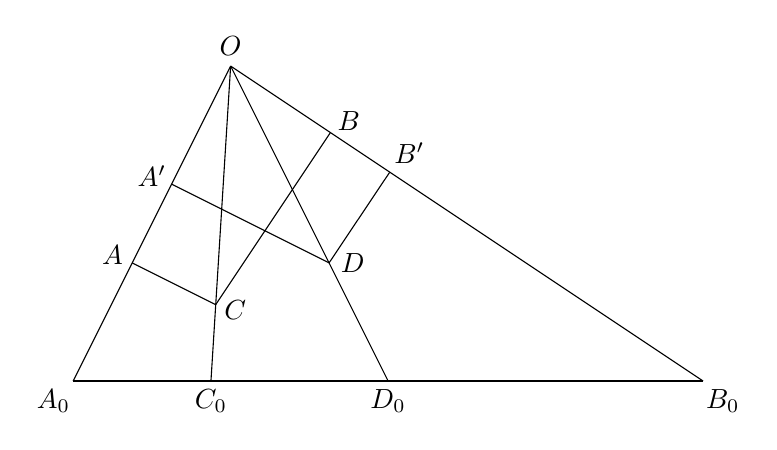
\begin{tikzpicture}
		\draw (-4,0) -- (4,0);
		\draw (-4,0) -- (-2,4); 
		\draw (-2,4) -- (4,0);
		\draw (-2,4) -- (0,0); 
		\draw (-2,4) -- (-2.25,0); 
		\draw (-3.25,1.5) -- (-2.19,0.97);
		\draw (-2.19,0.97) -- (-0.733,3.155);
		\draw (-2.75, 2.5) -- (-0.75,1.5);
		\draw (0.019, 2.65) -- (-0.75,1.5);

		\node at (-4.25,-0.25) {$A_0$};
		\node at (4.25,-0.25) {$B_0$};
		\node at (-2.25,-0.25) {$C_0$};
		\node at (0,-0.25) {$D_0$};
		\node at (-2,4.25) {$O$};
		\node at (-3.5, 1.6) {$A$};
		\node at (-3, 2.6) {$A'$};
		\node at (-0.5, 3.3) {$B$};
		\node at (0.27, 2.9) {$B'$};
		\node at (-0.45, 1.5) {$D$};
		\node at (-1.94, 0.9) {$C$};

	\end{tikzpicture}
	\end{center}
	From the definition, we have ${(a,b;c,d) = \frac{AC}{BC}\times\frac{B'D}{A'D}}$. Furthermore, from part (a), we have the result ${(A_0,B_0;C_0,D_0) = \frac{\sin(\angle{A_0OC_0}) \sin(\angle{B_0OD_0})}{\sin(\angle{B_0OC_0}) \sin(\angle{A_0OD_0})}}$. As we have right angled triangles, we get the following results from trigonometry.
	\begin{align*}
		\sin(\angle{A_0OC_0}) & = \frac{AC}{OC}, \hspace{10mm}
		\sin(\angle{B_0OD_0}) = \frac{B'D}{OD}\\
		\sin(\angle{B_0OC_0}) & = \frac{BC}{OD}, \hspace{10mm}
		\sin(\angle{A_0OD_0}) = \frac{A'D}{OC}
	\end{align*}
	Thus, we can rewrite the result from part (a) as 
	\begin{align*}
		(A_0,B_0;C_0,D_0) & = \frac{\sin(\angle{A_0OC_0}) \sin(\angle{B_0OD_0})}{\sin(\angle{B_0OC_0}) \sin(\angle{A_0OD_0})}\\
						  & = \frac{\left( \frac{AC}{OC} \times \frac{B'D}{OD} \right)}{\left( \frac{BC}{OC} \times \frac{A'D}{OD} \right)}\\
						  & = \frac{AC}{BC} \times \frac{B'D}{A'D}\\
						  & = (a,b;c,d)
	\end{align*}
	
	\pagebreak

\item Let $\ds{A, B, C, D}$ be distinct points on a (non-degenerate) conic section $\ds{\mathcal{C}}$ . If $\ds{O}$ is another point on $\ds{\mathcal{C}}$ and define lines $\ds{a, b, c, d}$ as in (b), show that the cross-ratio $\ds{(a, b; c, d)}$ does not depend on the point $\ds{O}$. (You may use the facts that every (non-degenerate) conic section is projectively equivalent to a circle and that a cross-ratio is unchanged by a projective transformation.)
	\bigbreak
	As every non-degenerate conic section is projectively equivalent to a circle, and the cross-ratio $\ds{(a,b;c,d)}$ is unchanged by a projective transformation, we only need to consider the case where $\ds{\mathcal{C}}$ is a circle. So, using the same notation as in part (b), we have the following configuration.

	\begin{center}
	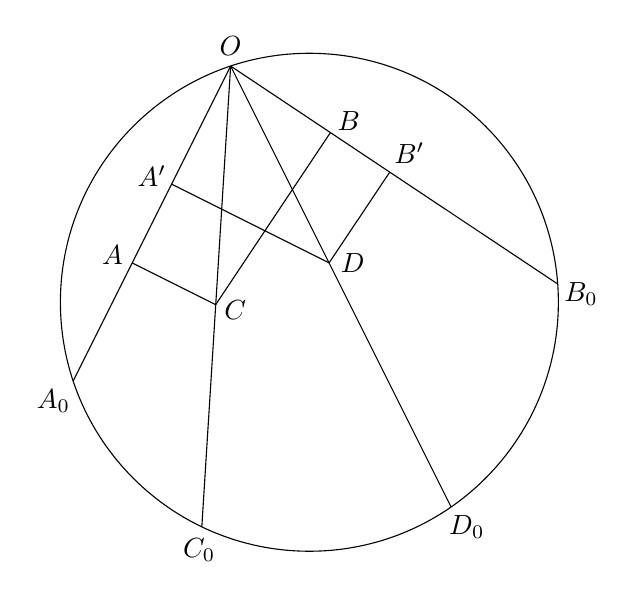
\begin{tikzpicture}
		\draw (-1,1) circle (3.162cm);
		\draw (-4,0) -- (-2,4); 
		\draw (-2,4) -- (2.154,1.231);
		\draw (-2,4) -- (0.8,-1.6); 
		\draw (-2,4) -- (-2.366,-1.852); 
		\draw (-3.25,1.5) -- (-2.19,0.97);
		\draw (-2.19,0.97) -- (-0.733,3.155);
		\draw (-2.75, 2.5) -- (-0.75,1.5);
		\draw (0.019, 2.65) -- (-0.75,1.5);

		\node at (-4.25,-0.25) {$A_0$};
		\node at (2.45,1.1) {$B_0$};
		\node at (-2.4,-2.15) {$C_0$};
		\node at (1,-1.85) {$D_0$};
		\node at (-2,4.25) {$O$};
		\node at (-3.5, 1.6) {$A$};
		\node at (-3, 2.6) {$A'$};
		\node at (-0.5, 3.3) {$B$};
		\node at (0.27, 2.9) {$B'$};
		\node at (-0.45, 1.5) {$D$};
		\node at (-1.94, 0.9) {$C$};

	\end{tikzpicture}
	\end{center}
	Consider the point $\ds{O'}$ on $\ds{\mathcal{C}}$, distinct from the point $\ds{O}$. Each angle in the cross-ratio formula derived in part (b) stands on an arc defined by two points from ${A_0,B_0,C_0,D_0}$. As arcs subtend equal angles at all points on the circumference, and considering the distinct points $\ds{O,O'}$, we get
	\begin{align*}
		\angle{A_0OC_0} & = \angle{A_0O'C_0}, \text{ } \angle{B_0OD_0} = \angle{B_0O'D_0}, \text{ } \angle{B_0OC_0} = \angle{B_0O'C_0}, \text{ } \angle{A_0OD_0} = \angle{A_0O'D_0}\\
		\therefore (a,b;c,d) & = \frac{\sin(\angle{A_0OC_0}) \sin(\angle{B_0OD_0})}{\sin(\angle{B_0OC_0}) \sin(\angle{A_0OD_0})} = \frac{\sin(\angle{A_0O'C_0}) \sin(\angle{B_0O'D_0})}{\sin(\angle{B_0O'C_0}) \sin(\angle{A_0O'D_0})}.
	\end{align*}
	Clearly, $\ds{(a,b;c,d)}$ does not depend on the point $\ds{O}$.

	\end{enumerate}
	\bigbreak
	\begin{center}
	\emph{This assignment is completely my own work except where acknowledged}\\
	\emph{signed:} \hspace{50mm} \emph{date:}\\
	\end{center}

	\end{enumerate}
\end{document}
